% IV-2-2 БД2 эцсийн тайлан. Хөрвүүлэх: cd report && xelatex IV-2-2_Final_Report.tex (2 удаа)
% Шаардлага: texlive-xetex, fonts-dejavu
\documentclass[11pt,a4paper]{article}
\usepackage{fontspec}
\setmainfont{DejaVu Serif}
\setsansfont{DejaVu Sans}
\setmonofont{DejaVu Sans Mono}[Scale=0.82]
\usepackage[margin=2.1cm]{geometry}
\usepackage{graphicx}
\usepackage{xcolor}
\usepackage{enumitem}
\usepackage{booktabs}
\usepackage{longtable}
\usepackage{array}
\usepackage{listings}
\usepackage{tikz}
\usetikzlibrary{arrows.meta,positioning,fit,backgrounds}
\usepackage{hyperref}
\usepackage{titlesec}
\usepackage{caption}
\usepackage{placeins}

\titleformat{\section}{\Large\bfseries}{\thesection.}{0.5em}{}
\titleformat{\subsection}{\large\bfseries}{\thesubsection}{0.5em}{}
\setlength{\parskip}{0.45em}
\setlength{\parindent}{0pt}
\sloppy
\setlength{\emergencystretch}{3em}
\hypersetup{colorlinks, linkcolor=blue!50!black, urlcolor=blue!50!black,
  pdftitle={IV-2-2 Final Report: Linux Kernel Module for Task Information}}
\captionsetup{font=small, labelfont=bf}
\graphicspath{{../docs/images/}{../src/ui/screenshots/}}

\lstset{
  basicstyle=\ttfamily\small, keywordstyle=\color{blue!70!black}\bfseries,
  commentstyle=\color{green!45!black}, stringstyle=\color{red!60!black},
  frame=single, framerule=0.3pt, rulecolor=\color{gray!60}, backgroundcolor=\color{gray!6},
  columns=fullflexible, keepspaces=true, language=C, showstringspaces=false,
  xleftmargin=0.5em, xrightmargin=0.5em, breaklines=true, escapeinside={(*@}{@*)}
}
\newcommand{\cyrcmt}[1]{\textcolor{green!45!black}{\ttfamily\small #1}}
\lstdefinestyle{out}{language={}, backgroundcolor=\color{black!3}}
\renewcommand{\contentsname}{Агуулга}
\renewcommand{\figurename}{Зураг}
\renewcommand{\tablename}{Хүснэгт}
\DeclareRobustCommand{\code}[1]{\texttt{\detokenize{#1}}}
\newcolumntype{L}[1]{>{\raggedright\arraybackslash}p{#1}}
% bare-metal үр дүн (tests/run_bd2.sh baremetal) ирэхээр бөглөнө
\newcommand{\TBDBM}{хүлээгдэж байна}
\newcommand{\TBDBMENV}{Bare-metal & Ubuntu 24.04.5 LTS (Dell Inspiron), kernel 7.0.0: үр дүн хүлээгдэж байна.\\}
\newcommand{\TBDBMBEFOREAFTER}{}

\begin{document}

%================================================================ Нүүр
\begin{titlepage}
\centering
\vspace*{0.4cm}
{\large\bfseries ШИНЖЛЭХ УХААН ТЕХНОЛОГИЙН ИХ СУРГУУЛЬ\\ МЭДЭЭЛЭЛ, ХОЛБООНЫ ТЕХНОЛОГИЙН СУРГУУЛЬ\par}
\vspace{1.6cm}

\includegraphics[height=3.6cm]{must_logo.png}\par
\vspace{2cm}
{\Huge\bfseries БИЕ ДААЛТ 2\\[4pt] ЭЦСИЙН ТАЙЛАН\par}
\vspace{0.5cm}
{\large\bfseries Үйлдлийн систем /F.CSM302/\par}
\vspace{2.4cm}
\begin{flushleft}
\renewcommand{\arraystretch}{1.3}
\begin{tabular}{@{}>{\raggedright\arraybackslash}p{5.2cm} >{\raggedright\arraybackslash}p{11cm}@{}}
\textbf{Сэдэв:} & ``Linux Kernel Module for Task Information. Programming Project 2 (3-р бүлэг), Task hierarchy''\\
\textbf{Хуваарилалтын код:} & IV-2-2\\
\textbf{Хувилбар:} & \code{v2.0.0}\\
\textbf{Хичээл заасан багш:} & Г.Ганбат /F.CS10/\\
\textbf{Гүйцэтгэсэн баг:} & Б.Төгөлдөр /B242270047/\\
 & С.Пүрэвтулга /B241940099/\\
 & Л.Пүрэв-очир /B232270108/\\
 & Б.Билгүүн /B190910014/\\
 & Л.Тэмүүлэн /B210930842/\\
 & Ч.Алтангэрэл /B231910003/\\
\end{tabular}
\end{flushleft}
\vfill
\begin{flushleft}
\begin{tabular}{@{}p{5.2cm} l@{}}
\textbf{Огноо:} & 2026 оны 11 дүгээр сарын 21\\
\end{tabular}
\end{flushleft}
\end{titlepage}

%================================================================ Хураангуй
\section*{Хураангуй}
\addcontentsline{toc}{section}{Хураангуй}

\textbf{Эцсийн шийдэл.} \code{pid.ko} kernel module нь \code{/proc/pid} файлаар PID хүлээн авч, номын форматаар task-ийн нэр, PID, төлөвийг, дараа нь эцэг болон хүүхдүүдийг хэвлэнэ. Вэб UI нь module-ийн гаралтаас процессын модыг зурж, туршилтын процессуудаар fork, stop, zombie, wait-ийг бодит цагт харуулна.

\textbf{Шүүмж.} Манай ажлыг шүүмжлэх IV-2-5 баг Review PDF ирүүлээгүй, Teams пост дээр техникийн comment ч ирээгүй. Тиймээс БД1-ийн тайланд өөрсдөө бичсэн хязгаарлалтууд болон кодыг kernel-ийн эх кодтой дахин тулгаж хийсэн self-review-ээс 10 шүүмж гаргасан (Major 3, Minor 4, Suggestion 3). Үүнээс 7-г зөвшөөрч зассан, 1-ийг хэсэгчлэн, 2-ыг үндэслэлтэйгээр татгалзсан.

\textbf{Гол сайжруулалт.} (1) Хүүхдийг RCU хамгаалдаггүй \code{task->children} жагсаалтаас биш, RCU-ээр хамгаалагдсан процессын жагсаалтаас олдог болсон. (2) Олон урсгалтай процессын бүх урсгалын хүүхдийг гаргаж, ppid нь \code{ps}-тэй ижил TGID болсон. (3) Нэг fd-ээр бичиж уншихад бусад процесс зэрэг бичсэн ч хариу холилдохгүй болсон. (4) UI \code{__state}-ийн битийг нэрээр нь тайлж, өвөг эцгийн гинжийг module-ээс авдаг болсон.

\textbf{Үр дүн.} Засвараас өмнөх \code{v1.0.1} module fork/exit ачааллын үед 21 секундэд \code{pid_show} дотор гацаж (soft lockup), kernel санах ойгоор дутаж VM унасан. v2 ижил ачаалалд 90 секунд, 17\,550 уншилтыг алдаагүй давсан. Зэрэг хандалтын тестэд нэг fd-ээр 20\,000 асуулгаас 0 зөрүү гарсан (v1: 7\,789). БД1-ийн бүх тест v2 дээр дахин давсан: basic 4/4 (WSL2-д 1 SKIP), boundary 7/7, regression 6/6, UI API 27 (1 алгассан), UI мод 12/12, интерфейсийн шалгагч 18 OK, 0 FAIL.

\newpage
\tableofcontents
\newpage

%================================================================ 1
\section{Төслийн тойм}

\textbf{Номын шаардлага.} Operating System Concepts (10-р хэвлэл) 3-р бүлгийн Programming Project 2: \code{/proc/pid} файл руу PID бичихэд module түүнийг хадгалж, уншихад тухайн task-ийн \code{command}, \code{pid}, \code{state}-ийг хэвлэнэ. Байхгүй PID бол юу ч хэвлэхгүй. Урьдчилсан нөхцөл нь 2-р бүлгийн \code{/proc} entry үүсгэдэг module.

\textbf{БД1-ийн үр дүн (\code{v1.0.1}).} Module номын бүх шаардлагыг хангаж, task hierarchy дүрслэлд зориулж \code{parent} ба \code{child} мөрийг нэмж хэвлэдэг байсан. Bare-metal Ubuntu 24.04 (kernel 7.0.0-34), Kubuntu 26.04.1 (kernel 7.0.0-38, Secure Boot) дээр basic 5/5, boundary 7/7, UI API 24 тест давсан.

\textbf{БД2-ын зорилго.} Шүүмжийг ангилж шийдвэрлэх, Major түвшний асуудлыг засах, засвар бүрийг шинэ тестээр нотлох, бичиг баримт, Poster, GitHub release-ийг эцэслэх.

\begin{center}
\begin{tabular}{L{3cm} L{12.5cm}}
\toprule
\textbf{Долоо хоног} & \textbf{Хийсэн ажил}\\
\midrule
11 & Self-review, ангилал, шийдвэр; module v2, UI засвар; regression тест (\code{tests/regression/}); WSL2 ба bare-metal дээр дахин туршилт\\
12 & Final Report, Manual, README, Poster, \code{v2.0.0} release, Teams-ийн ``БД2 - Final projects'' пост\\
\bottomrule
\end{tabular}
\end{center}

%================================================================ 2
\section{Эцсийн архитектур}

\begin{figure}[h]
\centering
\resizebox{\linewidth}{!}{%
\begin{tikzpicture}[
  box/.style={draw, rounded corners=3pt, align=center, minimum height=1cm, font=\small, fill=#1},
  box/.default=white, arr/.style={-{Stealth[length=2.2mm]}, thick}, lbl/.style={font=\scriptsize, align=center},
  chg/.style={draw=red!70!black, line width=1.2pt}]
  \node[box=blue!6, chg]   (br)  {Браузер\\\scriptsize app.js: \_\_state битүүд};
  \node[box=green!7, chg, right=1.6cm of br] (srv) {\code{server.py}\\\scriptsize нэг fd, өвөг эцэг module-ээс};
  \node[box=orange!10, right=1.6cm of srv] (proc) {\code{/proc/pid}\\\scriptsize fd бүрт \code{pid_ctx}};
  \node[box=red!8, chg, below=1.8cm of proc] (mod) {\code{pid.ko} v2\\\scriptsize proc\_open, proc\_write, pid\_show};
  \node[box=gray!12, below=1.8cm of srv, xshift=-1.3cm] (ts) {\code{task_struct}\\\scriptsize real\_parent, tasks жагсаалт};
  \node[box=gray!6, below=1.8cm of br] (pf) {\code{/proc/<pid>/stat}\\\scriptsize uid, урсгалын тоо};
  \draw[arr] (br) -- node[lbl, above]{GET /api/task\\?pid=N} (srv);
  \draw[arr] (srv) -- node[lbl, above]{open, write(N)\\lseek(0), read} (proc);
  \draw[arr] (proc) -- node[lbl, right]{kernel\\дуудалт} (mod);
  \draw[arr] (mod) -- node[lbl, below=2pt]{rcu\_read\_lock\\for\_each\_process} (ts);
  \draw[arr, dashed] (srv.south west) -- node[lbl, left, pos=0.4]{uid, урсгал} (pf.north east);
  \begin{scope}[on background layer]
    \node[draw, dashed, gray, fit=(mod)(ts), inner sep=8pt, label={[font=\scriptsize, gray]below:kernel space}] {};
  \end{scope}
\end{tikzpicture}}
\caption{Эцсийн бүтэц. Улаан хүрээтэй нь БД2-т өөрчлөгдсөн компонент.}
\end{figure}

\begin{center}
\begin{tabular}{L{4cm} L{11.5cm}}
\toprule
\textbf{Компонент} & \textbf{БД2-ын өөрчлөлт}\\
\midrule
\code{src/kmod/pid.c} & хүүхдийг \code{for_each_process} + \code{real_parent->tgid}-ээр (RCU); ppid = \code{task_tgid_vnr(real_parent)}; нээлт бүрт \code{struct pid_ctx}; \code{MODULE_VERSION("2.0")}\\
\code{src/ui/server.py} & \code{O_RDWR} нэг fd-ээр бичих, унших; \code{decode_state()}; өвөг эцгийн гинжийг module-ээс; PID 0-ийг татгалзана\\
\code{src/ui/static/app.js} & Мэдээллийн хүснэгт, зангилааны tooltip-д \code{__state}-ийн битийн нэр\\
\code{src/ui/contract_check.py} & OK / WARN / FAIL гаралт; нэг fd-ийн тусгаарлалтын шалгалт\\
\code{tests/regression/} & \code{fd_isolation.c}, \code{mt_fork.c}, \code{test_regression.sh} (R1--R6), \code{stress_compare.sh}, \code{bench_read.py}\\
\code{tests/run_bd2.sh} & v1.0.1 ба v2 module-ийг дараалан ачаалж бүх тестийг ажиллуулна\\
\bottomrule
\end{tabular}
\end{center}

\subsection{Module-ийн уншилт (v2)}
\begin{lstlisting}
rcu_read_lock();
task = pid_task(find_vpid(pid), PIDTYPE_PID);   (*@\cyrcmt{/* pid: энэ fd-ийнх эсвэл глобал */}@*)
if (!task)
        goto out;
seq_printf(m, "command = [%s] pid = [%d] state = [%u]\n",
           task->comm, task_pid_vnr(task), READ_ONCE(task->__state));
parent = rcu_dereference(task->real_parent);
if (pid_alive(task) && parent && parent != task)
        seq_printf(m, "parent = [%s] ppid = [%d]\n",
                   parent->group_leader->comm, task_tgid_vnr(parent));
if (!pid_alive(task))
        goto out;
for_each_process(p) {                            (*@\cyrcmt{/* tasks жагсаалт: RCU-ээр хамгаалагдсан */}@*)
        struct task_struct *rp = rcu_dereference(p->real_parent);
        if (p != task && rp && rp->tgid == task->tgid)
                seq_printf(m, "child = [%s] pid = [%d] state = [%u]\n",
                           p->comm, task_pid_vnr(p), READ_ONCE(p->__state));
}
out:
rcu_read_unlock();
\end{lstlisting}

\textbf{Яагаад \code{task->children}-ийг больсон бэ?} Kernel \code{children}/\code{sibling} жагсаалтыг \code{tasklist_lock}-оор хамгаалдаг: \code{fork} шинэ процессыг эцгийн жагсаалтад нэмэх, \code{exit} хүүхдүүдийг шинэ эцэг рүү шилжүүлэх, \code{wait} zombie-г устгах бүрд бичих түгжээ авна. Устгахдаа \code{list_del_init} хийдэг тул салгасан элемент өөр рүүгээ заана. Зөвхөн RCU-ийн дор гүйж байх үед яг тэр элемент дээр байвал гүйлт эцэс төгсгөлгүй эргэлдэнэ. Бид эхлээд \code{read_lock(&tasklist_lock)} авахаар төлөвлөсөн ч энэ түгжээ module-д export хийгдээгүй (\code{kernel/fork.c}-д зөвхөн \code{lockdep_tasklist_lock_is_held} export хийгддэг), \code{modpost} ``undefined'' гэж татгалзсан. Харин процессын үндсэн жагсаалт (\code{tasks}) \code{list_add_tail_rcu}, \code{list_del_rcu}-аар өөрчлөгддөг, \code{real_parent} нь \code{__rcu} заагч. Тиймээс бүх процессыг RCU-ийн дор гүйж эцгийн TGID-ээр шүүх нь module-аас хийж болох аюулгүй арга юм. \code{ps} болон \code{/proc/<pid>/stat}-ийн PPID ч яг ингэж (\code{real_parent}-ийн TGID) тооцогддог тул олон урсгалтай процессын асуудал (S2) мөн шийдэгдэнэ. Өртөг нь O(N): процесс бүрийг нэг удаа шалгана (§5.1-ийн хугацааны хэмжилт).

\subsection{Нээлт бүрийн PID (\code{pid_ctx})}
\code{proc_open} нь \code{kzalloc}-оор \code{struct pid_ctx}-ийг үүсгээд \code{single_open(file, pid_show, ctx)}-д дамжуулна. \code{proc_write} нь PID-ийг тухайн fd-ийн \code{ctx->pid} болон глобал \code{l_pid} хоёуланд бичнэ. \code{pid_show} нь энэ fd-ээр бичсэн PID байвал түүнийг, үгүй бол \code{l_pid}-ийг ашиглана. Ингэснээр:
\begin{itemize}[nosep]
  \item \code{echo N > /proc/pid; cat /proc/pid} (хоёр тусдаа нээлт) өмнөх шигээ ажиллана. Номын интерфейс өөрчлөгдөөгүй.
  \item \code{open(O_RDWR)}, \code{write}, \code{lseek(0)}, \code{read} хийвэл бусад процесс юу ч бичсэн өөрийн PID-ийн хариуг авна. UI сервер ингэж уншина.
\end{itemize}
\code{proc_release} нь \code{single_release}-ийн дараа \code{ctx}-ийг чөлөөлнө.

%================================================================ 3
\section{Туршилт ба дүрслэл}

\textbf{Орчин.}
\begin{center}
\begin{tabular}{L{3.2cm} L{12.3cm}}
\toprule
\textbf{Орчин} & \textbf{Тохиргоо}\\
\midrule
WSL2 (хөгжүүлэлт) & Windows 11, Intel Core i7-1255U, 3.9 GB RAM; Ubuntu 26.04 LTS, kernel \code{6.18.33.2-microsoft-standard-WSL2}, gcc 15.2, Python 3.14. Build орчныг \code{src/prereq/setup_wsl_kernel.sh}-ээр бэлтгэсэн. Kernel-ийг Microsoft gcc 13.2-оор хөрвүүлсэн тул symbol-ийн CRC зөрж, module-ийг \code{insmod -f}-ээр ачаалсан (\code{CONFIG_MODULE_FORCE_LOAD=y}, kernel ``F'' taint). v1 ба v2 хоёулаа ижил аргаар ачаалагдсан тул харьцуулалт шударга.\\
\TBDBMENV
\bottomrule
\end{tabular}
\end{center}

\textbf{Ажиглалтын урсгал.}
\begin{enumerate}[nosep]
  \item \code{sudo insmod src/kmod/pid.ko}, \code{python3 src/ui/server.py}, браузерт \code{http://localhost:8000}.
  \item \textbf{Demo мод үүсгэх}: \code{demo_root} болон S, R, T, Z төлөвтэй, 5 урсгалтай хүүхдүүд гарна. Мэдээллийн хүснэгтэд \code{__state = 8193} нь \code{TASK_INTERRUPTIBLE | TASK_FREEZABLE} гэж тайлагдана (Зураг \ref{fig:flags}).
  \item Зангилаа дээр хулганаа барихад tooltip-д тухайн процессын \code{__state} болон битүүд харагдана; \code{demo_stopped} нь \code{__TASK_STOPPED | TASK_WAKEKILL}.
  \item \textbf{Zombie}, \textbf{wait} товчоор хүүхэд Z болж, дараа нь алга болохыг ажиглана. ``Module дуудлагын лог''-д өвөг эцгийн гинжийг \code{/proc/pid}-ээс хэдэн удаа уншсан нь гарна.
  \item \code{tests/regression/mt_fork}-ийг ажиллуулаад түүний PID-ийг сонгоход үндсэн бус урсгалын fork хийсэн хүүхэд модонд гарна (Зураг \ref{fig:mt}).
  \item Терминалд \code{bash tests/regression/test_regression.sh}.
\end{enumerate}

%================================================================ 4
\section{Reviewer Responses}

Шүүмжийн эх сурвалж: \code{review/IV-2-2_Self_Review.md} (S1--S10). Оноогдсон баг (IV-2-5) шүүмж ирүүлээгүй, Teams-д comment ирээгүй.

{\small
\begin{longtable}{p{0.4cm} L{4.4cm} L{2.0cm} L{1.9cm} L{6.1cm}}
\toprule
\textbf{№} & \textbf{Шүүмж} & \textbf{Priority} & \textbf{Шийдвэр} & \textbf{Өөрчлөлт ба нотолгоо}\\
\midrule
\endhead
S1 & \code{children} жагсаалтыг зөвхөн RCU-ийн дор гүйлгэдэг; албан ёсоор \code{tasklist_lock} хамгаалдаг & Major & Зөвшөөрсөн & \code{tasklist_lock} module-д export хийгдээгүй тул хүүхдийг RCU-ээр хамгаалагдсан \code{for_each_process}-оор олдог болгосон (§2.1). v1: 21 секундэд soft lockup (\code{pid_show+0xda}), OOM, VM унасан. v2: 90 секунд, 17\,550 уншилт, алдаагүй (§5.1, \code{tests/bd2_wsl/stress_v*.txt}).\\
S2 & Олон урсгалтай процесс: үндсэн бус урсгалын хүүхэд дутуу, ppid нь TID & Major & Зөвшөөрсөн & Эцгийг TGID-ээр харьцуулж, \code{task_tgid_vnr}-ээр хэвлэнэ. R4, R5: v1 дээр FAIL (ppid 314 = TID), v2 дээр PASS (§5.1); Зураг \ref{fig:mt}.\\
S3 & Глобал \code{l_pid}: зэрэг ажиллахад хариу холилдоно & Major & Хэсэгчлэн & Номын echo/cat интерфейс хоёр тусдаа нээлт тул глобал PID-ийг устгах боломжгүй. Нэмэлтээр нээлт бүрт \code{pid_ctx}; UI түүнийг ашиглана. R3: v1 дээр нэг fd-ээр ч 7\,789/20\,000 зөрүү, v2 дээр 0/20\,000. Echo/cat горим v2-т ч холилдоно (13\,094), энэ нь номын интерфейсийн шинж.\\
S4 & UI PID 0-ийг зөвшөөрдөг, module татгалздаг & Minor & Зөвшөөрсөн & \code{parse_pid}: 1..4194304, ойлгомжтой мессеж. API test 05, 27.\\
S5 & \code{__state} тоог тайлдаггүй & Minor & Зөвшөөрсөн & \code{decode_state()} (16 бит), UI-ийн хүснэгт, tooltip. Test 25, 26; Зураг \ref{fig:flags}.\\
S6 & Өвөг эцгийн гинж procfs-оос & Minor & Зөвшөөрсөн & \code{parent} мөрийг дагаж module-ийг PID 1 хүртэл асууна. Test 03, 12; Зураг \ref{fig:flags}-ийн 4 өвөг эцэг.\\
S7 & README, Manual хуучирсан; шалгагчийн гаралтад тусгай тэмдэгт & Minor & Зөвшөөрсөн & README (БД2, шүүмжийн баг, Ubuntu 24.04, screenshot, regression), Manual, \code{contract_check} OK/WARN/FAIL.\\
S8 & \code{/proc/pid} 0666 эрхтэй & Suggestion & Зөвшөөрөөгүй & Номын даалгавар энгийн хэрэглэгч PID бичихийг шаарддаг. Гаргадаг мэдээлэл (comm, state, эцэг, хүүхэд) нь \code{/proc/<pid>/stat}-д аль хэдийн нээлттэй. Хэрэглэгчид бие биедээ саад болох асуудлыг S3-ын \code{pid_ctx} шийдсэн.\\
S9 & UI-д зориулсан \code{/proc/pid_tree} & Suggestion & Зөвшөөрөөгүй & Хамрах хүрээ: номын интерфейс нь \code{/proc/pid}. Шаардлагатай бүх өгөгдөл (task, эцэг, хүүхэд, өвөг эцэг) \code{/proc/pid}-ээс ирдэг болсон (S6). Хамгийн том (400 зангилаа) модыг ч 0.27--0.32 секундэд зурдаг тул гүйцэтгэлийн шалтгаан алга (§6).\\
S10 & Kernel < 5.14 дэмжихгүй & Suggestion & Зөвшөөрөөгүй & \code{__state} 5.14-д нэмэгдсэн. Ubuntu 22.04 (5.15), 24.04, 26.04 бүгд шинэ. \code{#if LINUX_VERSION_CODE} нэмбэл туршиж чадахгүй код үлдэнэ.\\
\bottomrule
\end{longtable}
}

%================================================================ 5
\section{Дахин туршилт}

\subsection{Засварын өмнө ба дараа}
Ижил компьютер дээр \code{tests/run_bd2.sh} нь эхлээд \code{v1.0.1} tag-ийн \code{pid.c}-г хөрвүүлж ачаалаад regression тестийг ажиллуулж, дараа нь v2-оор бүх тестийг ажиллуулна.

\begin{center}\small
\begin{tabular}{L{4.2cm} L{5.4cm} L{5.4cm}}
\toprule
\textbf{Тест} & \textbf{v1.0.1 (засварын өмнө)} & \textbf{v2.0 (засварын дараа)}\\
\midrule
R1 номын формат (echo/cat) & PASS & PASS\\
R2 \code{/sys/module/pid/version} & FAIL (хувилбаргүй) & PASS (2.0)\\
R3 тусдаа нээлт (echo/cat шиг) & 14\,893 / 20\,000 зөрүү & 13\,094 / 20\,000 зөрүү (номын горим, хүлээгдсэн)\\
R3 нэг fd, \code{lseek(0)} & 7\,789 / 20\,000 зөрүү, FAIL & 0 / 20\,000, PASS\\
R4 урсгалын fork хийсэн хүүхэд & жагсаалтад алга, FAIL & гарсан, PASS\\
R5 хүүхдийн ppid & 314 (урсгалын TID), \code{/proc}: 313, FAIL & 44 = TGID = \code{/proc}, PASS\\
R6 fork/exit ачаалал, 3000 уншилт & VM унасан (\code{E_UNEXPECTED}) & 3000/3000, dmesg цэвэр, PASS\\
\code{stress_compare.sh}, 90 сек & 4000 уншилтын дараа (21 сек) soft lockup, \code{pid_show+0xda}, OOM & 17\,550 уншилт, BUG/WARNING алга\\
Нэг уншилт, 25 процесс & 5.0--5.8 мкс (медиан) & 7.4--7.9 мкс\\
Нэг уншилт, 1025 процесс & 5.0--5.9 мкс & 47--56 мкс\\
\bottomrule
\end{tabular}
\end{center}

\begin{figure}[h!]
\centering
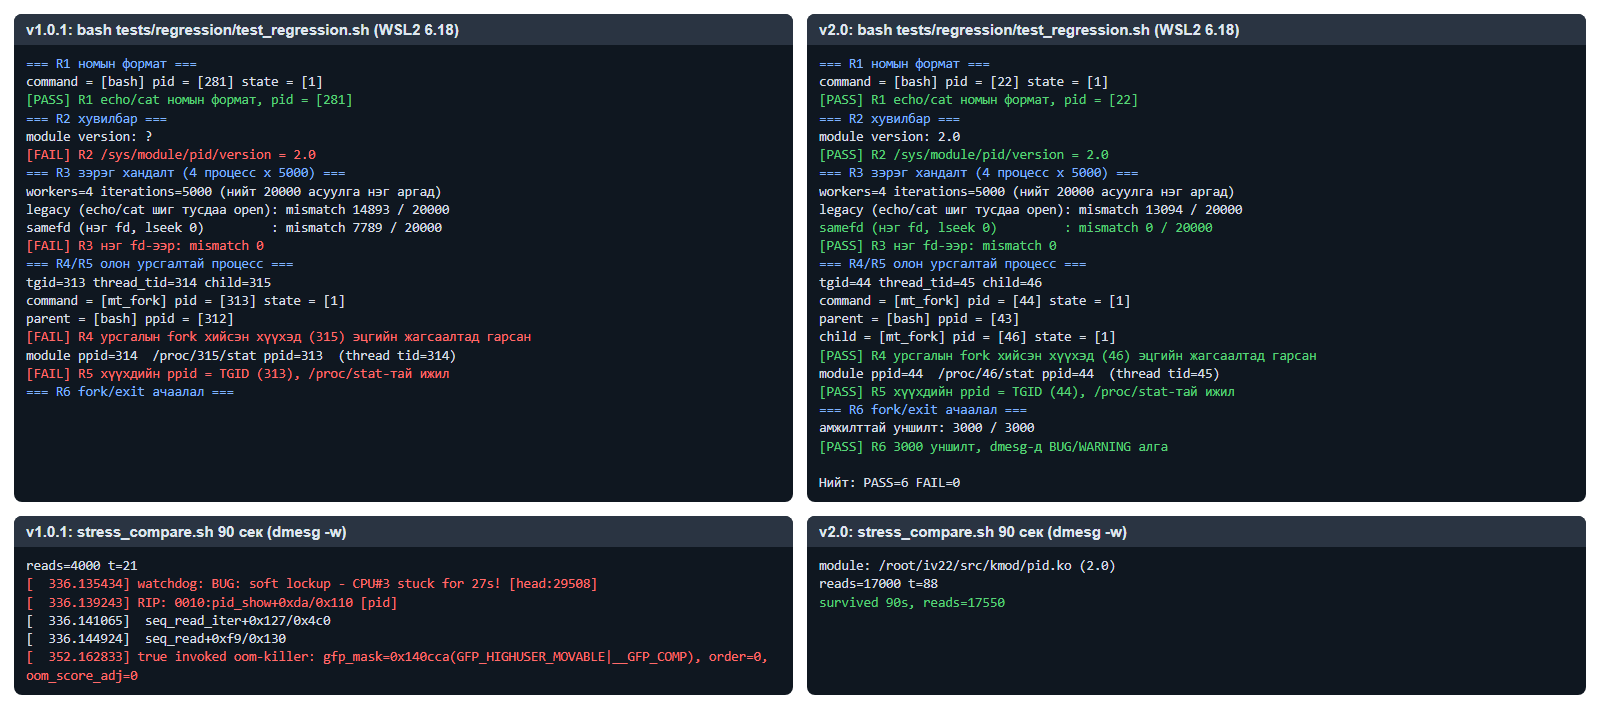
\includegraphics[width=\linewidth]{bd2_term_before_after.png}
\caption{Ижил компьютер, ижил скрипт: зүүн талд v1.0.1, баруун талд v2.0 (\code{tests/bd2_wsl/}-ийн бодит гаралт).}
\end{figure}

\textbf{Уналтын шинжилгээ.} v1 дээр R6-ийн үеэр WSL2 VM бүхэлдээ унасан тул \code{dmesg -w}-ийг Windows талын файл руу шууд бичдэг \code{stress_compare.sh}-ээр дахин үүсгэсэн. Kernel watchdog ``soft lockup - CPU\#3 stuck for 27s'' гэж, заагч нь \code{pid_show+0xda/0x110 [pid]} буюу \code{children} жагсаалтыг гүйх давталт дээр байгааг харуулсан. Хүүхэд устгагдах үед \code{list_del_init} элементийг өөр рүүгээ заалгадаг тул RCU-ийн дор гүйж буй уншигч тэндээ эргэлдэж, \code{seq_file} буфер нь дахин дахин томорсоор OOM болсон. v2-ийг ижил force load, ижил ачааллаар туршихад алдаа гараагүй тул уналт нь CRC-ийн зөрүүнээс биш, v1-ийн кодоос болсон гэж дүгнэв. Энэ нь БД1 тайланд ``ховор зөрүү гарч болзошгүй'' гэж бичсэн хязгаарлалт бодит, ноцтой алдаа байсныг харуулж байна.

\textbf{Гүйцэтгэлийн өртөг.} v2 хүүхдийг олохын тулд бүх процессыг гүйдэг тул уншилтын хугацаа процессын тооноос шугаман хамаарна: 1025 процесстой үед ~50 мкс. Энэ нь UI-ийн 1--5 секундын шинэчлэлтэд мэдэгдэхгүй бөгөөд kernel-ийг унагахаас хамаагүй дээр гэж үзэв.

\TBDBMBEFOREAFTER

\subsection{Regression}
БД1-ийн бүх тест (basic, boundary, UI API, contract) v2 module дээр дахин ажиллуулсан.

\begin{center}\small
\begin{tabular}{L{6.0cm} L{3.2cm} L{3.4cm} L{2.8cm}}
\toprule
\textbf{Тест} & \textbf{БД1 (v1.0.1, bare-metal)} & \textbf{v2.0, WSL2 6.18} & \textbf{v2.0, bare-metal}\\
\midrule
\code{tests/basic/test_basic.sh} & 5 PASS & 4 PASS, 1 SKIP\textsuperscript{a} & \TBDBM\\
\code{tests/boundary/test_boundary.sh} & 7 PASS & 7 PASS & \TBDBM\\
\code{tests/regression/test_regression.sh} & байгаагүй & 6 PASS & \TBDBM\\
\code{src/ui/tests/test_api.py} & 24 OK, 1 алгассан & 28 OK, 1 алгассан\textsuperscript{b} & \TBDBM\\
\code{src/ui/tests/test_tree.mjs} & 12 PASS & 12 PASS & \TBDBM\\
\code{src/ui/contract_check.py} & 17 зөв, 1 анхааруулга & 18 OK, 1 WARN\textsuperscript{c}, 0 FAIL & \TBDBM\\
\bottomrule
\end{tabular}
\end{center}
{\footnotesize a: WSL-ийн PID namespace-д kernel thread харагдахгүй (БД1-тэй ижил). b: \code{/proc/pid_tree}-тэй module шаарддаг тест (S9). c: \code{/proc/pid_tree} байхгүй (S9).}

\code{test_api.py}-ийн 3 шинэ тест (25--27) нэмэгдсэн. \code{test_12}-ийн хүлээлтийг шинэчилсэн: v2-т дуудлагын логт өвөг эцгийн гинжийг module-ээс асуусан мөр нэмэгдсэн тул 3 биш 4 мөр. Энэ нь S6-ийн хүлээгдсэн өөрчлөлт.

%================================================================ 6
\section{Эцсийн үр дүн}

\begin{center}\small
\begin{tabular}{L{6cm} L{9.5cm}}
\toprule
\textbf{Үзүүлэлт} & \textbf{Үр дүн}\\
\midrule
Major шүүмж (S1--S3) & 2 бүрэн, 1 хэсэгчлэн шийдсэн; гурвуулаа v1 дээр алдаатай, v2 дээр зөв гэж тестээр нотлогдсон\\
fork/exit ачаалалд тэсвэрлэх & v1: 21 сек; v2: 90 сек+ (17\,550 уншилт)\\
Зэрэг хандалт (нэг fd) & 0 / 20\,000 зөрүү\\
Олон урсгалтай процесс & хүүхэд гарна, ppid = TGID = \code{ps}\\
Нэг уншилт & 7--8 мкс (25 процесс), 47--56 мкс (1025 процесс)\\
UI: 400 зангилаатай мод & 275--318 мс (~630 процесс, 400 module асуулга)\\
UI: demo мод (8 зангилаа) & 5.8--7.9 мс\\
Автомат тест (v2, WSL2) & 4 + 7 + 6 + 27 + 12 = 56 давсан, 0 унасан (2 алгассан)\\
\bottomrule
\end{tabular}
\end{center}

\begin{figure}[h!]
\centering
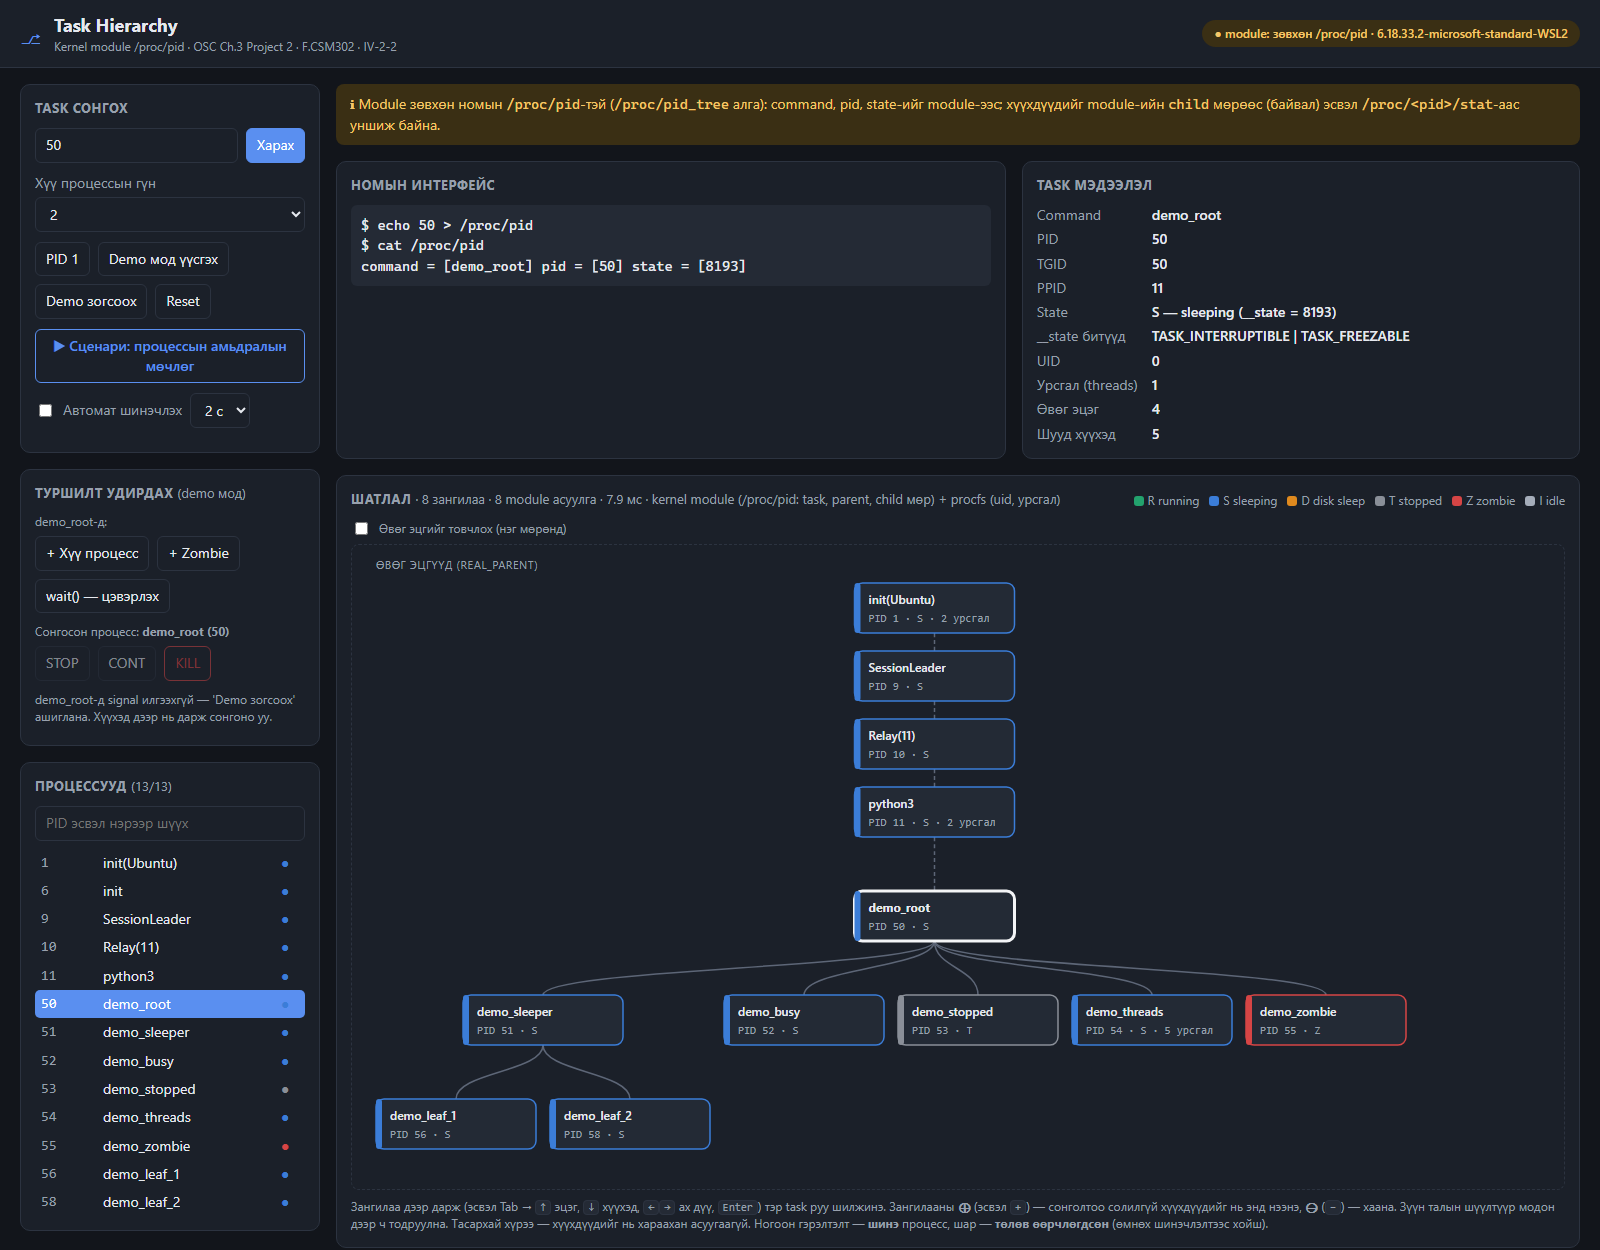
\includegraphics[width=\linewidth,height=0.42\textheight,keepaspectratio]{bd2_ui_demo_v2.png}
\caption{v2 UI: demo мод. ``\_\_state битүүд'' мөрөнд 8193 нь TASK\_INTERRUPTIBLE | TASK\_FREEZABLE; 4 өвөг эцгийг module-ээс асуусан (WSL2).}
\label{fig:flags}
\end{figure}

\begin{figure}[h!]
\centering
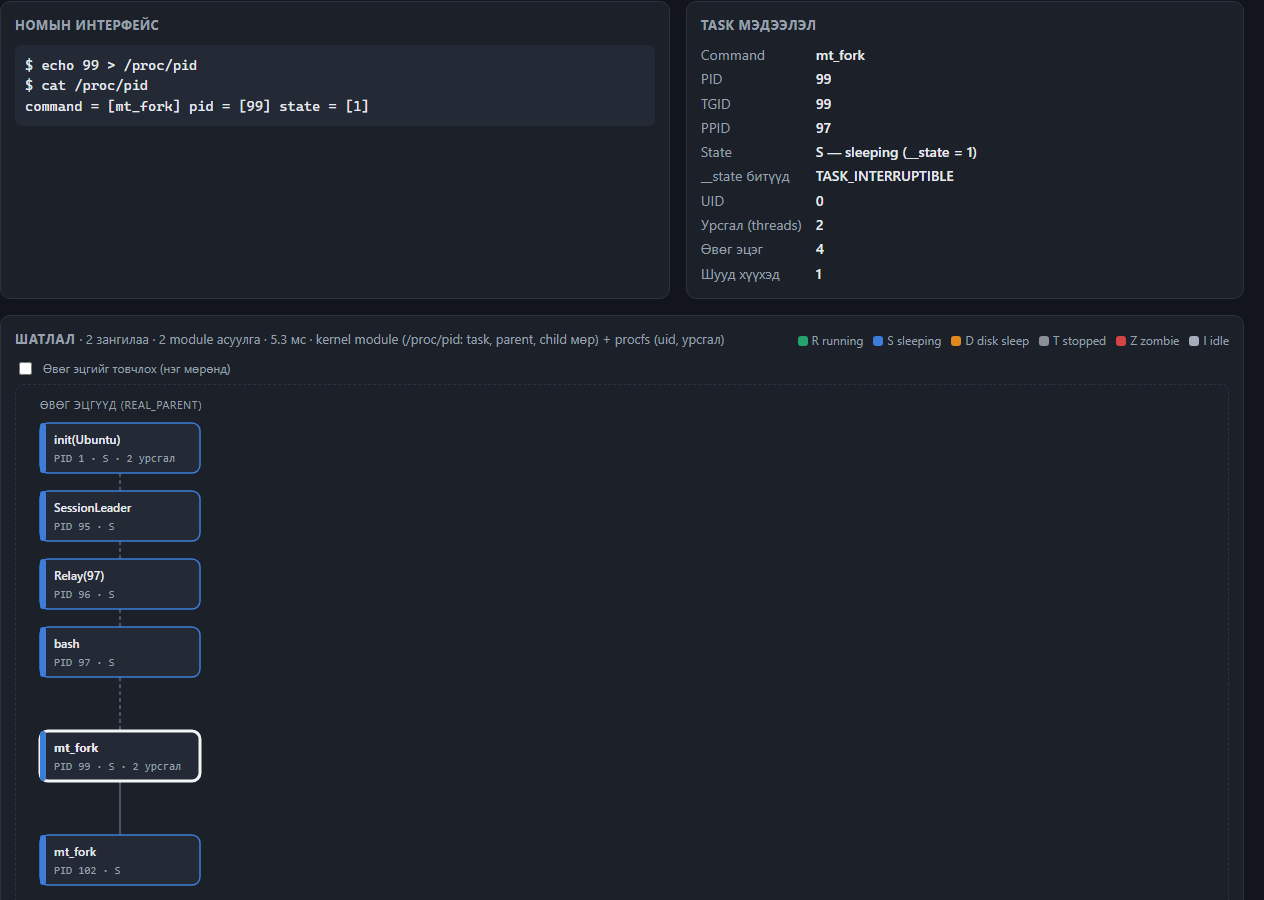
\includegraphics[width=0.85\linewidth,height=0.38\textheight,keepaspectratio]{bd2_ui_mt_fork.png}
\caption{\code{mt_fork} (2 урсгалтай): үндсэн бус урсгалын fork хийсэн хүүхэд (PID 102) модонд гарсан. v1 дээр энэ процесс хүүхэдгүй харагддаг байсан.}
\label{fig:mt}
\end{figure}
\FloatBarrier

%================================================================ 7
\section{Хязгаарлалт}
\begin{itemize}[nosep]
  \item Номын echo/cat горим глобал PID ашигладаг хэвээр тул терминалаас зэрэг бичвэл холилдож болно. Үүнээс сэргийлэх бол нэг fd-ээр уншина (Manual A5).
  \item \code{__state}-ийн битийн утга kernel-ийн хувилбараас хамаарна. \code{decode_state()} нь 6.x--7.0-ийн \code{include/linux/sched.h}-тай таарна; мэдэгдэхгүй битийг \code{0x...} гэж харуулна.
  \item UI тогтмол хугацаанд асуудаг тул хоёр шинэчлэлтийн хооронд үүсээд дууссан процесс харагдахгүй.
  \item Kernel 5.14-өөс хуучин хувилбар дээр хөрвүүлэгдэхгүй. Secure Boot асаалттай бол module-д гарын үсэг зурах шаардлагатай (Manual A3).
  \item WSL2-ийн Microsoft kernel-д \code{linux-headers} багц байхгүй тул \code{src/prereq/setup_wsl_kernel.sh}-ээр эх кодоос build орчин бэлтгэнэ (нэг удаа, удаан).
\end{itemize}

%================================================================ 8
\section{Дүгнэлт}
БД2-т манай ажилд гаднаас шүүмж ирээгүй ч өөрсдийн тайланд ``хязгаарлалт'' гэж бичээд орхисон зүйлсийг дахин шалгахад гурван нь бодит алдаа болж таарсан. Хамгийн чухал нь S1: v1 module fork/exit ачааллын үед kernel-ийг гацааж, санах ойг дуусгаж байсныг \code{dmesg}-ээр нотолж, RCU-ээр хамгаалагдсан процессын жагсаалт руу шилжүүлж зассан. Мөн олон урсгалтай процессын хүүхэд, зэрэг хандалтын асуудлыг шийдэж, засвар бүрийг өмнө/дараах тестээр баталгаажуулсан. Номын интерфейс (\code{echo}, \code{cat}, гаралтын формат) өөрчлөгдөөгүй, БД1-ийн бүх тест хэвээр давж байна.

Суралцсан зүйл: kernel-ийн өгөгдлийн бүтэц бүр өөрийн түгжээтэй бөгөөд RCU бүх жагсаалтыг хамгаалдаггүй; module-аас аль түгжээг ашиглаж болохыг export хийгдсэн symbol тодорхойлдог; ``ховор тохиолддог'' уралдааны нөхцөлийг ачааллын тестээр хэдхэн секундэд илрүүлж болно. Эцсийн код, тест, бичиг баримт \code{v2.0.0} release-д байна.

%================================================================ Материал
\section*{Ашигласан материал}
\addcontentsline{toc}{section}{Ашигласан материал}
\begin{enumerate}[nosep, label={[\arabic*]}]
  \item A. Silberschatz, P. B. Galvin, G. Gagne. \emph{Operating System Concepts}, 10th ed. Wiley, 2018. 3-р бүлэг (Programming Project 2), 7-р бүлэг (readers-writers).
  \item Linux kernel source: \code{kernel/fork.c} (\code{copy_process}), \code{kernel/exit.c} (\code{forget_original_parent}), \code{include/linux/sched.h}, \code{include/linux/sched/signal.h}. \url{https://elixir.bootlin.com/linux/}
  \item The Linux Kernel documentation: ``The seq\_file interface'', ``What is RCU?''. \url{https://docs.kernel.org/}
  \item IV-2-2 БД1 тайлан ба Manual, \code{v1.0.1}. \url{https://github.com/Tugu8/os-bd1-IV-2-2-/releases/tag/v1.0.1}
\end{enumerate}

\clearpage
\appendix
%================================================================ A
\section{Сайжруулалтын бүртгэл}
{\small
\begin{longtable}{p{0.4cm} L{3.1cm} L{2.0cm} L{2.2cm} L{3.8cm} L{3.3cm}}
\toprule
\textbf{№} & \textbf{Шүүмж} & \textbf{Priority} & \textbf{Шийдвэр} & \textbf{Хийсэн өөрчлөлт} & \textbf{Нотолгоо}\\
\midrule
\endhead
1 & S1 RCU ба \code{children} & Major & Зөвшөөрсөн & \code{pid_show}: \code{for_each_process}, \code{real_parent->tgid} & R6, \code{stress_v1/v2.txt}\\
2 & S2 олон урсгал & Major & Зөвшөөрсөн & ppid = \code{task_tgid_vnr}; бүх урсгалын хүүхэд & R4, R5, Зураг \ref{fig:mt}\\
3 & S3 глобал \code{l_pid} & Major & Хэсэгчлэн & \code{struct pid_ctx}, \code{proc_open/release}; UI \code{O_RDWR} & R3, contract ``Нэг fd''\\
4 & S4 PID 0 & Minor & Зөвшөөрсөн & \code{parse_pid} 1..4194304 & test 05, 27\\
5 & S5 \code{__state} & Minor & Зөвшөөрсөн & \code{decode_state}, UI мөр, tooltip & test 25, 26, Зураг \ref{fig:flags}\\
6 & S6 өвөг эцэг & Minor & Зөвшөөрсөн & \code{_module_ancestors} & test 03, 12\\
7 & S7 баримт бичиг & Minor & Зөвшөөрсөн & README, Manual, CHANGELOG, OK/WARN/FAIL & PR\\
8 & S8 0666 & Suggestion & Үгүй & (номын шаардлага) & §4\\
9 & S9 \code{/proc/pid_tree} & Suggestion & Үгүй & (хамрах хүрээ) & §4, §6\\
10 & S10 kernel < 5.14 & Suggestion & Үгүй & (туршиж чадахгүй) & §4\\
\bottomrule
\end{longtable}
}

\begin{center}\small
\begin{tabular}{L{4.6cm} L{3.6cm} L{3.6cm} L{3.6cm}}
\toprule
\textbf{Тест} & \textbf{Засварын өмнө} & \textbf{Засварын дараа} & \textbf{Дүгнэлт}\\
\midrule
fork/exit ачаалал & 21 сек, soft lockup & 90 сек, алдаагүй & S1 шийдэгдсэн\\
Олон урсгалтай процесс & хүүхэд алга, ppid = TID & хүүхэд гарна, ppid = TGID & S2 шийдэгдсэн\\
Зэрэг хандалт, нэг fd & 7\,789 зөрүү & 0 зөрүү & S3 шийдэгдсэн (fd горимд)\\
Зэрэг хандалт, echo/cat & 14\,893 зөрүү & 13\,094 зөрүү & номын интерфейсийн шинж, Manual A9\\
UI PID 0 & module EINVAL, ойлгомжгүй & 400, ``1-ээс эхэлнэ'' & S4\\
\bottomrule
\end{tabular}
\end{center}

\end{document}
